\documentclass[12pt]{article}
\author{Lawrence Liu}
\usepackage{subcaption}
\usepackage{graphicx}
\usepackage{amsmath}
\usepackage{pdfpages}
\newcommand{\Laplace}{\mathscr{L}}
\setlength{\parskip}{\baselineskip}%
\setlength{\parindent}{0pt}%
\usepackage{xcolor}
\usepackage{listings}
%\definecolor{backcolour}{rgb}{0.95,0.95,0.92}
\usepackage{amssymb}
\usepackage[T1]{fontenc}
\usepackage{beramono}%\lstdefinestyle{mystyle}{
%    backgroundcolor=\color{backcolour}}
%\lstset{style=mystyle}
%\usepackage[usenames,dvipsnames]{xcolor}%%
%% Julia definition (c) 2014 Jubobs
%%



\title{ECE 133A HW 1}
\begin{document}
\maketitle
\section*{Exercise T2.4}
$\phi$ is not linear, since point 2 is equal to the negative of point 3, but the output of the function
at point 2 is not the negative of the output at point 3.
\section*{Exercise T2.8}
\subsection*{(a)}
\begin{align*}
\int p(x)dx&=\sum_{i=1}^{n}c_i\frac{1}{i}x^{i}\\
\int_{\alpha}^\beta&=\sum_{i=1}^{n}c_i\frac{1}{i}(\beta^i-\alpha^i)
\end{align*}
therefore we have
$$a=\boxed{\left((\beta-\alpha)),...,\frac{1}{n}(\beta^n-\alpha^n)\right)}$$
\subsection*{(b)}
we have
$$p'(\alpha)=\sum_{i=1}^{n}(i-1)c_i \alpha^{i-2}$$
thus we get
$$b=\boxed{\left(0,1,...,(n-1)\alpha^{n-2}\right)}$$
\section*{Exercise A1.2}
let $u=(\sqrt{x_1},...,\sqrt{x_n})$ and $v=\left(\sqrt{\frac{1}{x_1}},...,\sqrt{\frac{1}{x_n}}\right)$, from Cauchy-Schwarz we have
\begin{align*}
	\|u^Tv\|&\leq \|u\|\|v\|\\
	\|u^Tv\|^2&\leq \|u\|^2\|v\|^2\\
	n^2&\leq\left(\sum_{k=1}^{n}x_n\right)\left(\sum_{k=1}^{n}\frac{1}{x_k}\right)\\
	\frac{1}{n}\sum_{k=1}^{n}x_k&\geq n\left(\sum_{k=1}^n\frac{1}{x_k}\right)^{-1}\\
	\frac{1}{n}\sum_{k=1}^{n}x_k&\geq\left(\frac{1}{n}\sum_{k=1}^n\frac{1}{x_k}\right)^{-1}\\
\end{align*}
\section*{Exercise T3.25}
\subsection*{(a)}
\begin{align*}
	E[p]&=\boxed{\theta\mu+(1-\theta)\mu^{\text{rf}}\textbf{1}}
\end{align*}
\begin{align*}
	Var(p)&=\theta^2\sigma^2\\
	\sqrt{Var(p)}&=\boxed{|\theta|\sigma}
\end{align*}
\subsection*{(b)}
Therefore we have that 
$$\theta_{optimal}=\pm \frac{\sigma^{\text{tar}}}{\sigma}$$
Therefore if our risky asset has a possitive rate of return, we will pick
$$\theta_{optimal}=\boxed{\frac{\sigma^{\text{tar}}}{\sigma}}$$
And if our risky asset has a negative rate of return we will choose
$$\theta_{optimal}=\boxed{-\frac{\sigma^{\text{tar}}}{\sigma}}$$
\subsection*{(c)}
If we want our portfolio to have a lower risk level than the asset, ie $\sigma^{\text{tar}}<\sigma$,
but if the expected return rate of the asset is still positive, then we will hedge,
since $\theta_{optimal}=\frac{\sigma^{\text{tar}}}{\sigma}<1$.\\\\
If we are comfortable with a greater level of risk than the asset, ie $\sigma^{\text{tar}}>\sigma$, and
if the expected return rate of the asset is still positive, we will Leverage
since $\theta_{optimal}=\frac{\sigma^{\text{tar}}}{\sigma}>1$.\\\\
And, if the expected return rate of the asset is negative, we will short the asset.
\section*{Exercise A1.10}
After 29 iterations, I get a $J^{\text{cluster}}=34.63$ and clusters which look like this
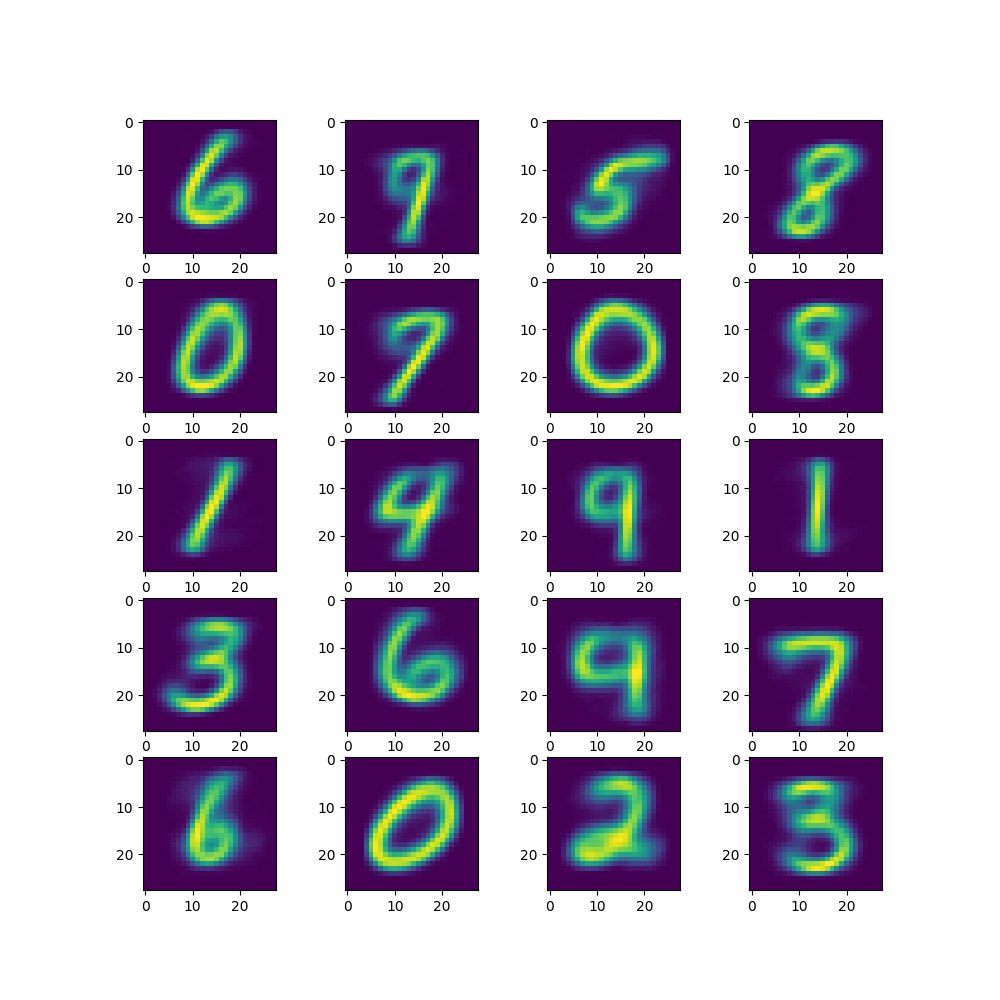
\includegraphics[scale=0.5]{digits.png}
This was acomplished with the following code in Julia
\lstinputlisting[
    basicstyle=\tiny, %or \small or \footnotesize etc.
]{Kmeans.jl}
\end{document}
